\documentclass[10pt,twocolumn]{article}

\usepackage[utf8]{inputenc}
\usepackage[T1]{fontenc}
\usepackage[english]{babel}
\usepackage{cite}
\usepackage{times}
\usepackage[margin=2cm]{geometry}
\usepackage{titlesec}
\usepackage{hyperref}
\usepackage{booktabs}
\usepackage{enumitem}
\usepackage{tikz}
\usetikzlibrary{arrows.meta, positioning, fit, backgrounds, shapes.geometric}

\titleformat{\section}{\normalfont\large\bfseries}{\thesection}{1em}{}
\titleformat{\subsection}{\normalfont\normalsize\bfseries}{\thesubsection}{1em}{}
\titleformat{\subsubsection}{\normalfont\normalsize\bfseries}{\thesubsubsection}{1em}{}
\setlength{\columnsep}{0.5cm}

\title{\Large\bfseries MARley: A ChatBot for Academic Advising in the M.Sc. Computer Science Program at Philipps-Universit\"at Marburg}
\author{Bachelor Thesis Proposal by:\\
Joshua Tobias Hoffmann\\
\small Philipps-Universit\"at Marburg -- Department of Mathematics and Computer Science\\
\small Supervised by: Prof. Dr. Christin Seifert, Van Bach Nguyen -- Explainable Artificial Intelligence Group\\
\small Planned registration date: 16.03.2026\\
\small \texttt{hoffma6z@students.uni-marburg.de}}
\date{}

\begin{document}
\maketitle

% =============================================================================
\section{Introduction}
% =============================================================================

% --- Part 1: The Problem ---
Students in higher education programs regularly need to access study-related information such as admission criteria, module requirements, credit point allocations, and examination deadlines. This information is typically contained in formally structured documents --- the Studien- und Pr\"ufungsordnung (StPO, study and examination regulations), module handbooks, and university websites --- that are often lengthy and contain legal paragraphs with cross-references to other sections and annexes, as well as complex table structures. Understanding and correctly interpreting this information requires familiarity with the underlying regulatory structure and its terminology. As a consequence, students face considerable search effort and an elevated risk of misinterpreting or overlooking relevant rules. This burden extends to advisory offices and lecturers, who frequently receive and answer recurring questions about the same regulatory topics.

% --- Part 2: RAG as Solution ---
Chatbots capable of providing reliable, source-grounded responses represent a promising approach to address this problem: they can reduce the workload on advisory offices while giving students immediate and reliable access to their questions. Retrieval-Augmented Generation (RAG) is a framework that is particularly well suited for this purpose, as it augments the generation process with externally provided knowledge sources~\cite{lewis2021rag}. A RAG system operates in two stages: first, a \emph{retrieval} component searches the external knowledge base --- such as study regulations or FAQ documents --- to identify text passages relevant to the user's query; second, a \emph{generation} component, typically a large language model (LLM), produces an answer that is grounded in the retrieved evidence rather than relying solely on the model's internal knowledge. In the university context, this means that a RAG-based chatbot can access examination regulations, module handbooks, or FAQ documents and provide information based on that, rather than merely reproducing general knowledge. However, RAG does not completely eliminate the risk of hallucinations~\cite{ji2023hallucination}: the generation model may still produce plausible but factually unsupported statements. This risk makes two additional requirements essential: Every answer must include references to its sources. If the retrieved evidence is insufficient or contradictory, the system must \emph{abstain} — explicitly communicating that its knowledge is too limited to provide a reliable answer — and refer the student to the appropriate advisory contact, rather than generating potentially incorrect information.

% =============================================================================
\section{Objective and Goals}
% =============================================================================

\subsection{Objective}
This thesis will develop \textbf{MAR}ley (\textbf{MAR}burg Study Advising ChatBot), a modular RAG system for the M.Sc. Computer Science program at Philipps-Universit\"at Marburg. Using RAG as its architectural foundation, the thesis will design, implement, and evaluate a complete pipeline --- from source preprocessing and chunking through retrieval and generation to controlled abstention. MARley shall provide factually accurate, source-grounded answers to student queries about the StPO. It shall be able to determine whether the retrieved evidence is insufficient and transparently abstain from responding rather than providing unsupported information. The pipeline architecture will be designed to be modular, so that individual components can be evaluated independently and be replaced without affecting the remaining system.

\subsection{Goals}
The objectives of this thesis address the individual modules of the chatbot pipeline: first, the preparation of the knowledge base; second, the analysis of various retrieval strategies; and third, the implementation of a suitable abstention method to prevent incorrect output.

\medskip
\noindent\textbf{G1: Knowledge Preparation and Chunking.}
The knowledge base of MARley will be built upon two primary sources in this thesis: the StPO of the Master's program, and an FAQ comprising authentic student questions along with the corresponding responses from the advisory office (FAQ-AO). These sources differ fundamentally in structure: the StPO constitutes a long document with sections, annexes, and tables, while the FAQ consists of short, self-contained question--answer pairs. Therefore, in a preparatory step, the complex format of the StPO shall be processed by leveraging an LLM to derive a synthetic FAQ from the original source, which will serve as a third source within the chatbot's knowledge base (FAQ-StPO). In the subsequent retrieval step, two different chunking strategies shall be applied for the retrieval of sources. This is necessary, as a single chunking strategy cannot adequately accommodate all source formats --- chunks that are too large dilute retrieval precision, while chunks that are too small lose necessary context. These complementary chunking strategies will be implemented: (a)~\emph{sliding-window chunking} for the StPO PDF, which splits the text into overlapping, sentence-aligned windows of configurable size, preserving context across paragraph boundaries; and (b)~\emph{FAQ chunking}, which treats each question--answer pair as a self-contained retrieval unit. The parameters of both strategies (window size, overlap, token budget) shall be tuned so that downstream retrieval can reliably cover the range of typical student queries.

\medskip
\noindent\textbf{G2: Retrieval Strategy Comparison.}
Student queries vary widely in type: some are specific factual look-ups (e.g., ``How many ECTS does the thesis count for?''), while others are broader questions about regulations or procedures (e.g., ``What are the admission criteria for a specific module?''). Therefore, the second objective of this thesis is to identify and implement a retrieval strategy which covers the widest possible range of queries. Three different retrieval methods shall be implemented in the chatbot pipeline either individually or in combination: \emph{BM25}, a sparse retrieval method~\cite{robertson2009bm25}; \emph{vector retrieval}, a dense retrieval method; and \emph{hybrid retrieval} using Reciprocal Rank Fusion (RRF)~\cite{cormack2009rrf}. The comparison aims to determine which strategy --- or combination --- delivers the highest evidence quality across different query categories.

\medskip
\noindent\textbf{G3: Generation and Controlled Abstention.}
In academic advising, factually incorrect answers can have direct consequences for students --- for example, wrong information about deadlines, admission criteria, or module prerequisites may lead to missed registrations or incorrect study plans. The third goal of this thesis addresses this risk by focusing on the configuration of the generation process such that it (a)~produces answers that are faithful to the retrieved evidence, (b)~cites its sources transparently so that students can verify the information, and (c)~abstains explicitly when the retrieved evidence is insufficient or contradictory. In the case of abstention, the system shall communicate that it cannot provide a reliable answer and, where applicable, refer the student to the appropriate advisory contact (e.g., the advisory office or the examination office).

% =============================================================================
\section{Related Work}
% =============================================================================

Retrieval-Augmented Generation (RAG) combines a retrieval component with a generative language model: given a query, relevant passages are first retrieved from an external knowledge base, and the language model then generates an answer conditioned on these passages~\cite{lewis2021rag}. This two-stage approach allows the system to ground its responses in external evidence rather than relying solely on the model's parametric knowledge, which is particularly important for knowledge-intensive question answering. Surveys show that the specific design of the retrieval strategy, context construction, and response control mechanisms is decisive for the factual accuracy of the generated answers~\cite{gao2024ragsurvey}.
Several RAG-based chatbots for university advising have been developed in recent years. \emph{Marcel}~\cite{trienes2025marcel} is a conversational agent for prospective students of Master programs at Philipps-Universit\"at Marburg that retrieves information from curated program descriptions. \emph{JayBot}~\cite{odede2024jaybot} targets course and admission queries at a UK university using GPT-3.5 with vector search; preliminary user studies report high satisfaction but do not evaluate factual accuracy systematically. \emph{URAG}~\cite{nguyen2025urag} proposes a two-tiered architecture that routes queries through an enriched FAQ tier before falling back to full document retrieval. \emph{BarkPlug~v.2}~\cite{neupane2024barkplug} applies RAGAS-based evaluation to a campus resource chatbot at Mississippi State University. A recent survey by Swacha and Gracel~\cite{swacha2025ragsurvey} covers 47~RAG chatbots in education and identifies hallucination mitigation, evaluation methodology, and domain adaptation as recurring open problems. However, none of these systems specifically target \emph{StPO} --- formally structured legal documents with cross-references, annexes, and tables that require structure-preserving extraction and domain-specific chunking strategies.

The following subsections review the individual techniques that MARley will build upon: retrieval methods, structure-preserving preprocessing, hallucination mitigation, and evaluation frameworks.

Retrieval methods play a crucial role in enabling access to diverse source formats. BM25~\cite{robertson2009bm25} --- a probabilistic ranking function based on term frequency and document length --- remains a strong baseline for sparse, keyword-based retrieval. For queries that require semantic understanding beyond exact keyword overlap, dense retrieval methods based on text embeddings have shown complementary strengths. Hybrid fusion approaches such as Reciprocal Rank Fusion (RRF)~\cite{cormack2009rrf} combine sparse and dense retrieval rank lists into a single merged rank, exploiting the strengths of both paradigms.

For formal documents containing tables, hierarchies, and cross-references, structure-preserving preprocessing is essential for downstream retrieval quality. Work on document understanding benchmarks confirms that layout and structural information carry important signals that are lost by naive text extraction~\cite{borchmann2021due}. This is directly relevant to MARley, where the StPO contains complex table structures and cross-references between sections and annexes that must be preserved during extraction.

The frequency of hallucinations is particularly critical to the value of a source-based chatbot. Instances where a language model generates fluent but factually incorrect or unsupported text remain a relevant risk even in RAG systems~\cite{ji2023hallucination}. Several strategies have been proposed to mitigate this problem. For instance, R-Tuning~\cite{zhang2024rtuning} is a method that instructs models to respond with ``I don't know'' when sufficient evidence is lacking, thereby demonstrating improved calibration in safety-critical contexts.

The development of a RAG-based chatbot pipeline requires continuous evaluation of the output in order to assess and adjust the architecture. RAGAS~\cite{es2025ragas} provides an established framework for evaluating RAG systems along three dimensions: \emph{Context Relevance} (whether the retrieved passages are pertinent to the query), \emph{Faithfulness} (whether the generated answer is supported by the retrieved context), and \emph{Answer Relevance} (whether the answer addresses the original question). Linking these automated metrics to domain-specific failure categories --- for example, incorrect deadlines, wrong ECTS values, or missing prerequisites --- remains an open challenge for advising systems.

% =============================================================================
\section{Architecture}
% =============================================================================

To realize the goals defined in Section~2, MARley will be designed as a modular pipeline in which each stage corresponds to one or more of these goals and can be developed, evaluated, and replaced independently. Figure~\ref{fig:architecture} provides an overview of this pipeline.

\begin{figure}[ht]
\centering
\resizebox{0.88\columnwidth}{!}{%
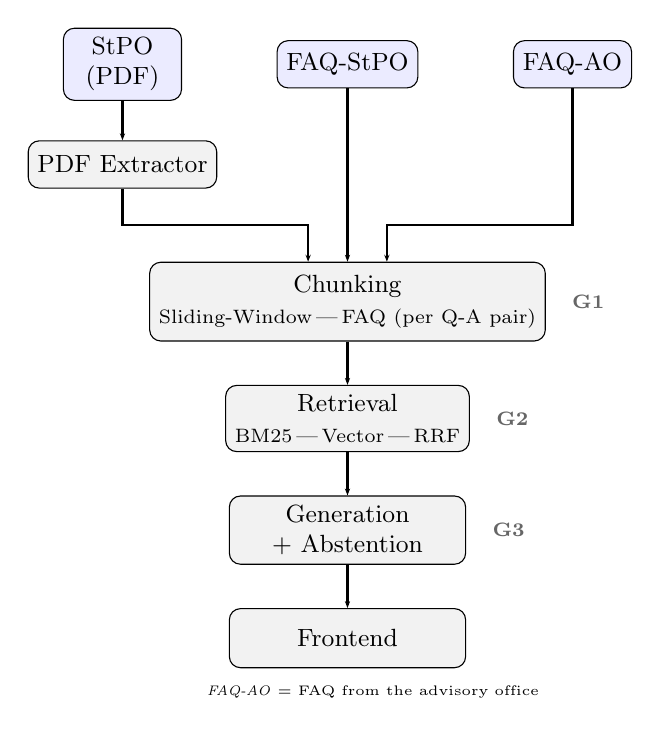
\begin{tikzpicture}[
    node distance=0.55cm,
    every node/.style={font=\small},
    stage/.style={draw, rounded corners, minimum height=0.75cm, minimum width=3cm, align=center, fill=gray!10},
    source/.style={draw, rounded corners, minimum height=0.6cm, minimum width=1.5cm, align=center, fill=blue!8},
    smallstage/.style={draw, rounded corners, minimum height=0.6cm, minimum width=2cm, align=center, fill=gray!10, font=\small},
    glabel/.style={font=\scriptsize\bfseries, text=black!60, anchor=west},
    arr/.style={-{Stealth[length=2.5pt]}, thick}
  ]
  % --- Row 1: Sources ---
  \node[source] (faqpdf) {FAQ-StPO};
  \node[source, left=1.2cm of faqpdf] (pdf) {StPO\\(PDF)};
  \node[source, right=1.2cm of faqpdf] (faqao) {FAQ-AO};

  % --- PDF Extractor below PDF ---
  \node[smallstage, below=0.5cm of pdf] (extractor) {PDF Extractor};

  % --- Chunking (showing both strategies) ---
  \node[stage, below=2.2cm of faqpdf, minimum height=1cm] (chunking) {Chunking\\{\scriptsize Sliding-Window\,|\,FAQ (per Q-A pair)}};

  % --- Retrieval ---
  \node[stage, below=0.55cm of chunking] (retrieval) {Retrieval\\{\scriptsize BM25\,|\,Vector\,|\,RRF}};

  % --- Generation ---
  \node[stage, below=0.55cm of retrieval] (generation) {Generation\\+ Abstention};

  % --- Frontend ---
  \node[stage, below=0.55cm of generation] (frontend) {Frontend};

  % --- Goal labels ---
  \node[glabel] at ([xshift=6pt]chunking.east) {G1};
  \node[glabel] at ([xshift=6pt]retrieval.east) {G2};
  \node[glabel] at ([xshift=6pt]generation.east) {G3};

  % --- Arrows ---
  \draw[arr] (pdf) -- (extractor);
  \path (extractor.south) -- (chunking.north) coordinate[midway] (midroute);
  \draw[arr] (extractor.south) -- (extractor.south |- midroute) -| ([xshift=-5mm]chunking.north);
  \draw[arr] (faqpdf) -- (chunking);
  \draw[arr] (faqao.south) -- (faqao.south |- midroute) -| ([xshift=5mm]chunking.north);
  \draw[arr] (chunking) -- (retrieval);
  \draw[arr] (retrieval) -- (generation);
  \draw[arr] (generation) -- (frontend);

  % --- Legend ---
  \node[anchor=north west, font=\tiny, text width=5cm, inner sep=2pt, align=left]
    at ([yshift=-4pt, xshift=-10pt]frontend.south west) {%
      \textit{FAQ-AO} = FAQ from the advisory office%
    };

\end{tikzpicture}%
}
\caption{MARley pipeline. Labels indicate the goal evaluated at each stage.}
\label{fig:architecture}
\end{figure}

The knowledge base will draw on three complementary sources: the StPO of the study program, a synthetic FAQ derived from this regulation (FAQ-StPO), and an FAQ compiled from authentic student questions by the advisory office (FAQ-AO). Since the StPO is distributed as a PDF containing structured formal elements such as tables, cross-references, and annexes, a dedicated PDF extractor will first parse the document into a structured JSON representation that preserves these elements for downstream processing. The implementation will use PyMuPDF~\cite{pymupdf_docs} and pdfplumber~\cite{pdfplumber_repo} for PDF extraction.

To feed the knowledge base data into the retrieval process, all sources will need to be segmented into units small enough for precise matching yet large enough to preserve meaningful context. Since the three sources differ fundamentally in structure, a single chunking strategy cannot serve both formats adequately. Therefore, two complementary strategies will be applied: \emph{sliding-window chunking} will split the JSON structure of the StPO into overlapping, sentence-aligned windows of configurable size, preserving context across paragraph boundaries; \emph{FAQ chunking} will treat each question--answer pair as a self-contained retrieval unit, producing compact, high-precision chunks. Both strategies will produce chunks that are stored in a shared index. Sentence segmentation will be performed with syntok~\cite{syntok_repo}, and token counting with tiktoken~\cite{tiktoken_repo}.

In response to a user query, the retrieval component will identify the most relevant chunks from the shared index. As student queries range from specific keyword-based look-ups to broader semantic questions about regulations and procedures, no single retrieval method is likely to perform optimally across all query types. The pipeline will therefore implement three strategies: BM25~\cite{robertson2009bm25} for sparse, keyword-based retrieval (using rank-bm25~\cite{rank_bm25_pypi}), vector retrieval for dense, embedding-based matching (using ChromaDB~\cite{chroma_docs}), and hybrid retrieval using Reciprocal Rank Fusion (RRF)~\cite{cormack2009rrf}, which merges the ranking lists of both methods into a single combined result. Chunks from all three knowledge sources will compete on equal terms in the retrieval ranking; source prioritization will be handled through rank fusion rather than through rigid preprocessing rules.

The generation component will receive the top-ranked chunks as output from the retrieval stage and produce an answer grounded exclusively in this retrieved evidence. A locally hosted LLM served via Ollama~\cite{ollama_api_docs} will power the generation, returning structured metadata including source references and confidence indicators. This will ensure that answers remain transparent and verifiable. In academic advising, an incorrect answer can be more harmful than no answer at all. For this reason, the pipeline will include a controlled abstention mechanism: when the retrieved evidence is insufficient or contradictory, the system will communicate explicitly that it cannot provide a reliable answer rather than generating potentially incorrect information.

A web-based frontend built with FastAPI~\cite{fastapi_docs} will serve as the interface between the pipeline and the user. It will display the generated answer together with its source references and confidence metadata, enabling students to verify the information independently.

% =============================================================================
\section{Evaluation}
% =============================================================================

A systematic evaluation is necessary to determine whether the individual pipeline components and the system as a whole meet the goals defined in Section~2. The evaluation will follow the pipeline structure and address each goal with dedicated metrics. The aim is to test the individual components --- chunking, retrieval, and generation/abstention --- in various configurations and to assess their impact on the quality of the responses.

The evaluation dataset will comprise approximately 100~questions with reference answers, drawn systematically from two complementary sources. The first source will be the set of FAQs whose content is derived from the StPO (FAQ-StPO), covering formal topics such as admission criteria, module requirements, ECTS, and deadlines. The second source will consist of FAQs compiled by the advisory office (FAQ-AO), which reflect frequently asked real-world student questions --- including procedural, cross-referencing, and edge-case queries that are typically harder to answer from the regulations alone. To ensure varying retrieval difficulty and to test different system capabilities, the dataset will be stratified into three categories:
\begin{itemize}[leftmargin=1.2em]
    \item \emph{Direct look-up} questions answerable from a single chunk (e.g., ``How many ECTS does the thesis count for?''),
    \item \emph{Multi-source} questions requiring evidence from multiple sections or sources (e.g., ``Which modules can I take without prerequisites in my first semester?''),
    \item \emph{Unanswerable} questions for which the knowledge base contains no or insufficient evidence, designed to test abstention behavior.
\end{itemize}

For evaluation of MARley's retrieval component, standard metrics will be used. This includes \emph{Precision@$k$} (the proportion of the top-$k$ retrieved passages that are relevant), \emph{Recall@$k$} (the proportion of all relevant passages that appear in the top-$k$ results), and \emph{Mean Reciprocal Rank} (MRR, the reciprocal of the rank at which the first relevant passage appears). The comparison will be conducted across all three question categories to reveal whether different strategies have systematic strengths or weaknesses for particular query types --- for example, keyword-heavy factual look-ups versus semantically broader regulation questions.

The quality of the generation component will be evaluated along two dimensions: factuality and abstention behavior. For factuality, the RAGAS framework~\cite{es2025ragas} provides three automated metrics: Context Relevance measures whether the retrieved passages are pertinent to the query; Faithfulness measures whether the generated answer is supported by the retrieved context; and Answer Relevance measures whether the answer addresses the original question. Both FAQ-StPO and FAQ-AO questions will be used for this evaluation. Abstention will be assessed separately using the unanswerable questions in the dataset: the system should abstain on these questions and should \emph{not} abstain on answerable ones. Abstention precision (the proportion of abstained responses that were indeed unanswerable) and abstention recall (the proportion of unanswerable questions on which the system correctly abstained) will be reported to quantify how reliably the system distinguishes answerable from unanswerable queries.

A combined end-to-end evaluation will assess how well MARley provides correct, source-traceable, and appropriately abstaining answers across all question categories and pipeline configurations.

% =============================================================================
\section{Discussion}
% =============================================================================

Beyond the quantitative evaluation, several design decisions and inherent limitations of the system warrant closer examination. The discussion will address trade-offs between answer completeness and factual safety --- that is, the tension between providing comprehensive information and avoiding incorrect statements. A further topic includes the transferability of the pipeline architecture to other study programs or universities.

% =============================================================================
\section{Outlook and Conclusion}
% =============================================================================

While the core of this thesis focuses on the design, implementation, and evaluation of the MARley pipeline (G1--G3), the modular architecture opens up several directions for future work. Upon successful implementation and evaluation of the core goals, two optional extensions are considered: first, an investigation of how PDF extraction quality influences downstream retrieval and generation performance; and second, an extended automatic evaluation using the full RAGAS metric suite to identify additional failure patterns beyond the core metrics. In the longer term, the modular architecture is designed to support extension to additional degree programs and the replacement of individual pipeline components --- for example, upgrading the PDF extractor or substituting the embedding model for vector retrieval.

% =============================================================================
\section{Timeline}
% =============================================================================

\begin{table}[ht]
\centering
\small
\begin{tabular}{@{}l p{7,5cm}@{}}
\toprule
\textbf{Weeks} & \textbf{Phase} \\
\midrule
1--2   & Scope definition, evaluation criteria, stabilizing data basis \\
3--5   & Chunking variants, retrieval strategies (BM25, vector, RRF) \\
6--8   & Generation, abstention logic, frontend integration \\
9--10  & Evaluation run ($\sim$100 questions), analysis and error classification \\
11--12 & Writing, finalization, and proofreading \\
\bottomrule
\end{tabular}
\end{table}

% =============================================================================
\section{Disclosure of GenAI Tool Usage}
% =============================================================================

Generative AI was used for literature screening, linguistic revision, and \LaTeX{} formulation. Conceptualization, implementation, and evaluation are carried out independently by the author.

\newpage
\bibliographystyle{plain}
\bibliography{related-work}

\end{document}
